\documentclass{beamer}

\usepackage[utf8]{inputenc}
\usepackage[T1]{fontenc}
\usepackage{amsmath}
\usepackage{amssymb}
\usepackage{amsthm}
\usepackage{graphicx}
\usepackage{hyperref}
\usepackage{booktabs}
\usepackage{bm}
\usepackage{enumerate}
\usepackage{tikz}
\usepackage{tikz-3dplot}
\usepackage{tikz-cd}
\usetikzlibrary{math}
\usetikzlibrary{cd}

% Mathematical commands
\newcommand{\E}{\mathbb{E}}
\newcommand{\R}{\mathbb{R}}
\newcommand{\N}{\mathbb{N}}
\newcommand{\C}{\mathbb{C}}
\newcommand{\I}{\mathbf{I}}
\newcommand{\NN}{\mathcal{N}}
\newcommand{\norm}[1]{\left\lVert#1\right\rVert}
\newcommand{\abs}[1]{\left\lvert#1\right\rvert}
\newcommand{\evmin}[1]{\lambda_{\min}\left(#1\right)}
\newcommand{\evmax}[1]{\lambda_{\max}\left(#1\right)}
\newcommand{\svmin}[1]{\sigma_{\min}\left(#1\right)}
\newcommand{\tr}{\text{tr}}
\newcommand{\KNTK}{K_{\text{NTK}}}
\newcommand{\Kinf}{K^{\infty}}
\newcommand{\Sd}{\mathbb{S}^{d-1}}
\newcommand{\Lap}{\Delta}
\newcommand{\Ls}{\mathcal{L}_s}
\newcommand{\limiting}[1]{#1^{\infty}}

\usetheme{Madrid}
\usecolortheme{default}

\title{Spectral Analysis of the Neural Tangent Kernel}
\subtitle{And its Modification by Sobolev-type Training}
\author{Synthesis and Analysis}
\date{\today}

\begin{document}

\begin{frame}
\titlepage
\end{frame}

\begin{frame}{Outline}
\tableofcontents
\end{frame}






\begin{frame}{Sobolev training eigen scaling laws and learning}
\textbf{Key objectives:}
\begin{itemize}
\item Obtain NTK's operator eigenvalues scaling laws with respect to decay rate: $\mu_\ell \sim \ell^{-\alpha}$
\item Then understand spectral properties of Sobolev training
\item Also Derive scaling laws for sampled NTK matrix eigenvalues w.r.t. network depth $l$ and data size $n$
\end{itemize}

Warning : The NTK matrix is a sampled version of the NTK operator with our dataset. Its eigenvalues are not the same as the NTK operator's eigenvalues.

Initialization : 
\begin{itemize}
\item \textbf{Edge of Chaos:} Initialize weights as $w_{ij} \sim \mathcal{N}(0, \sigma_w^2/\text{fan-in})$ where $\sigma_w^2 = 2$ 
for ReLU networks to maintain unit variance through layers
\end{itemize}
\end{frame}




\begin{frame}{Example NTK Matrix Structure}
Consider a dataset of 3 points $x_1, x_2, x_3 \in \mathbb{R}^d$. The NTK matrix has entries:
\[
K^{\infty} = \begin{pmatrix} 
k(x_1,x_1) & k(x_1,x_2) & k(x_1,x_3) \\
k(x_2,x_1) & k(x_2,x_2) & k(x_2,x_3) \\
k(x_3,x_1) & k(x_3,x_2) & k(x_3,x_3)
\end{pmatrix}
\]
where $k(x_i,x_j)$ is the NTK kernel function. For general depth $l$ networks at EOC:
\[
K^{\infty}(\mathbf{x}_1, \mathbf{x}_2) = \|\mathbf{x}_1\| \|\mathbf{x}_2\| \left( \sum_{k=1}^l \varrho^{\circ (k-1)}\left(\rho_1^{\infty}(\mathbf{x}_1, \mathbf{x}_2)\right) \prod_{k'=k}^{l-1} \varrho'\left(\varrho^{\circ (k'-1)}\left(\rho_1^{\infty}(\mathbf{x}_1, \mathbf{x}_2)\right)\right) \right) \mathbf{I}_{m_l}
\]

For 2 layers ReLU networks, this simplifies to:
\[
k(x_i,x_j) = x_i^T x_j \cdot \arccos(-\langle x_i,x_j \rangle) + \sqrt{1-\langle x_i,x_j \rangle^2}
\]

\end{frame}


\begin{frame}{NTK Operator Structure}
Consider functions $f,g \in L^2(\Sd)$. The NTK operator acts as:
\[
(\Kinf f)(x) = \int_{\Sd} k(x,y)f(y)dy
\]
where $k(x,y)$ is the same NTK kernel.

\textbf{Key Properties:}
\begin{itemize}
\item Symmetric positive definite operator
\item Eigenfunctions are spherical harmonics
\item Eigenvalues decay polynomially: $\mu_\ell \sim \ell^{-\alpha}$
\end{itemize}
\end{frame}







\begin{frame}{Visualization of Points on $\mathbb{S}^1$}
\begin{center}
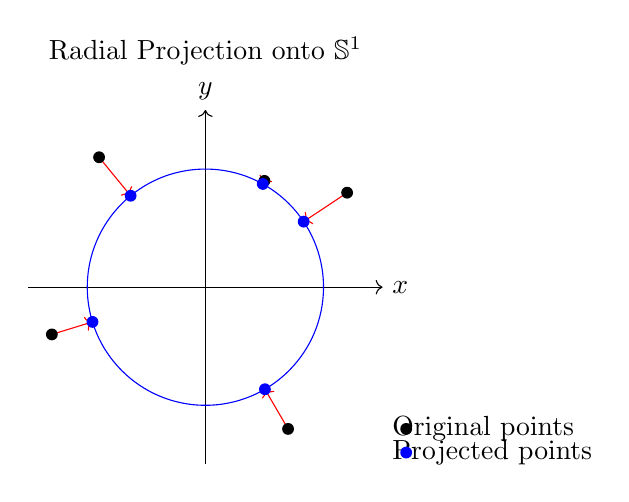
\begin{tikzpicture}[scale=1.5]
    % Draw coordinate axes
    \draw[->] (-1.5,0) -- (1.5,0) node[right] {$x$};
    \draw[->] (0,-1.5) -- (0,1.5) node[above] {$y$};
    
    % Draw the unit circle
    \draw[blue] (0,0) circle (1);
    
    % Draw 10 points with their projections
    % Point 1 (from (1.2, 0.8) to normalized)
    \draw[red,->] (1.2,0.8) -- (0.832,0.555);
    \fill (1.2,0.8) circle (0.05);
    \fill[blue] (0.832,0.555) circle (0.05);
    
    % Point 2 (from (-0.9, 1.1) to normalized)
    \draw[red,->] (-0.9,1.1) -- (-0.633,0.774);
    \fill (-0.9,1.1) circle (0.05);
    \fill[blue] (-0.633,0.774) circle (0.05);
    
    % Point 3 (from (-1.3, -0.4) to normalized)
    \draw[red,->] (-1.3,-0.4) -- (-0.956,-0.294);
    \fill (-1.3,-0.4) circle (0.05);
    \fill[blue] (-0.956,-0.294) circle (0.05);
    
    % Point 4 (from (0.7, -1.2) to normalized)
    \draw[red,->] (0.7,-1.2) -- (0.504,-0.864);
    \fill (0.7,-1.2) circle (0.05);
    \fill[blue] (0.504,-0.864) circle (0.05);
    
    % Point 5 (from (0.5, 0.9) to normalized)
    \draw[red,->] (0.5,0.9) -- (0.486,0.874);
    \fill (0.5,0.9) circle (0.05);
    \fill[blue] (0.486,0.874) circle (0.05);
    
    % Add legend
    \node[right] at (1.5,-1.2) {Original points};
    \fill (1.7,-1.2) circle (0.05);
    \node[right] at (1.5,-1.4) {Projected points};
    \fill[blue] (1.7,-1.4) circle (0.05);
    
    % Add title
    \node[above] at (0,1.8) {Radial Projection onto $\mathbb{S}^1$};
\end{tikzpicture}
\end{center}
\begin{itemize}
\item Points in $\R^2$ projected radially onto $\mathbb{S}^1$
\item Represents sampling from radial distribution
\end{itemize}
\end{frame}






\begin{frame}{Matrix Spectrum Results}
\begin{itemize}
\item \textbf{Condition Number:}
  \[ \kappa(K^{\infty}) \sim 1 + \frac{n}{3} + \mathcal{O}(n \xi / l) \]
  Grows linearly with data size $n$, improves with depth $l$

\item \textbf{Eigenvalue Distribution:}
  \[ \lambda_{\text{min}} \sim \frac{3l}{4}, \quad \lambda_{\text{max}} \sim \frac{3nl}{4} \pm \xi \text{ where } \xi \sim \log(l) \]
  Minimum scales linearly with depth, maximum scales with both depth and data size

What dictate the training is the NTK matrix eigenvalues.

\item \textbf{Applicability:} Valid for all Leaky ReLU activation functions
\end{itemize}

\textbf{Key Takeaway:} Deeper networks ($l \uparrow$) improve conditioning but with diminishing returns
\end{frame}

\begin{frame}{NTK-Sobolev Operator}
    \begin{center}
    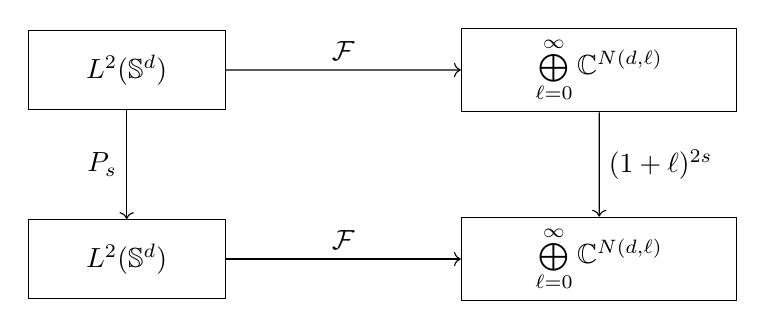
\begin{tikzpicture}[scale=1.2]
        % Draw the main boxes
        \node (A) at (0,2) [draw, minimum width=2.5cm, minimum height=1cm] {$L^2(\mathbb{S}^d)$};
        \node (B) at (5,2) [draw, minimum width=3.5cm, minimum height=1cm] {$\bigoplus\limits_{\ell=0}^{\infty} \mathbb{C}^{N(d,\ell)}$};
        \node (C) at (0,0) [draw, minimum width=2.5cm, minimum height=1cm] {$L^2(\mathbb{S}^d)$};
        \node (D) at (5,0) [draw, minimum width=3.5cm, minimum height=1cm] {$\bigoplus\limits_{\ell=0}^{\infty} \mathbb{C}^{N(d,\ell)}$};
        
        % Draw the arrows
        \draw[->] (A) -- node[above] {$\mathcal{F}$} (B);
        \draw[->] (A) -- node[left] {$P_s$} (C);
        \draw[->] (B) -- node[right] {$(1+\ell)^{2s}$} (D);
        \draw[->] (C) -- node[above] {$\mathcal{F}$} (D);
    \end{tikzpicture}
    \end{center}

    \vspace{0.5em}
    \textbf{Spherical Harmonics Transform:} $\mathcal{F}$ maps functions to their spectral decomposition
    
    \end{frame}



\begin{frame}{From Sobolev Loss to Fourier Space Operator}
\textbf{Sobolev loss with gradients:}
\[ \mathcal{L}_s[f] = \|f\|_{L^2}^2 + \|\nabla f\|_{L^2}^2 = \int_{\Sd} f(x)^2 d\sigma(x) + \int_{\Sd} \|\nabla f(x)\|^2 d\sigma(x) \]

\textbf{Fourier decomposition:} $f(x) = \sum_{\ell,p} \hat{f}_{\ell,p} Y_{\ell,p}(x)$
\[ \mathcal{L}_s[f] = \sum_{\ell=0}^{\infty} \sum_{p=1}^{N(d,\ell)} (1+\ell)^{2s} |\hat{f}_{\ell,p}|^2 \]

\textbf{Discretization at points $\{x_i\}_{i=1}^n$:}
\[ \hat{f}_{\ell,p} \approx \sum_{i=1}^n c_i f(x_i) Y_{\ell,p}(x_i) \]

\textbf{Matrix form:} $P_s = \sum_{\ell,p} (1+\ell)^{2s} a_{\ell,p} a_{\ell,p}^T$
where $(a_{\ell,p})_i = c_i Y_{\ell,p}(x_i)$

\textbf{Final form:} $\mathcal{L}_s[f] \approx f^T P_s f$ with $f = (f(x_1), \ldots, f(x_n))^T$
\end{frame}


    \begin{frame}{NTK-Sobolev Operator}
    \textbf{Spectral Coefficients:}
    \[ (a_{\ell,p})_i = c_iY_{\ell,p}(x_i) \]

    \vspace{0.3em}
    \textbf{NTK-Sobolev Norm:}
    \[ \Phi_s(W) = \frac{1}{2}(y-u)^\top P_s(y-u) \]

    \begin{alertblock}{Key Insight}
        The NTK-Sobolev operator eigenvalues determine the Fourier spectrum of learned functions.
    \end{alertblock}
    
    \textbf{Dimension Growth:}
    \[ N(d,\ell) \sim \frac{2\ell^{d-2}}{(d-2)!} \quad \text{as } \ell \to \infty \]
\end{frame}





\begin{frame}{Regularity Results}
\begin{theorem}[ReLU Network Regularity]
For a 2-layer ReLU network $N: \Sd \to \R$:
\begin{itemize}
\item $N \in H^s(\Sd)$ for all $s < 3/2$
\item For $s \geq 3/2$, $N \in H^s(\Sd)$ if and only if $N$ is affine
\end{itemize}
\end{theorem}
and the spectrum scales as:
\[ \lambda_k \sim k^{2s} \quad \text{as } k \to \infty \]

So we chose s to compensate the decay of the NTK operator eigenvalues.
\item Eigenvalues decay: $\mu_\ell = \mathcal{O}(\ell^{-d})$
\end{frame}

\begin{frame}{Discretized Sobolev Loss}
\begin{equation*}
\Phi_s(W) = \frac{1}{2} \sum_{\ell=0}^{\ell_{\max}} \sum_{p=1}^{N(d,\ell)} (1+\ell)^{2s} \left|\sum_{i=1}^n c_i Y_{\ell,p}(x_i)(g-N)(x_i)\right|^2
\end{equation*}
\begin{itemize}
\item Equivalent matrix form:
\[ \Phi_s(W) = \frac{1}{2}(y-u)^\top P_s(y-u) \]
where $P_s = \sum_{\ell=0}^{\ell_{\max}} \sum_{p=1}^{N(d,\ell)} (1+\ell)^{2s}P_{\ell,p}$
\item And:
\[ P_s = \sum_{\ell=0}^{\ell_{\max}} \sum_{p=1}^{N(d,\ell)} (1+\ell)^{2s}P_{\ell,p}, \quad P_{\ell,p} = a_{\ell,p}a_{\ell,p}^\top, \quad (a_{\ell,p})_i = c_iY_{\ell,p}(x_i) \]
\end{itemize}
\textbf{Asymptotic growth:}
\[ N(d,\ell) \sim \frac{2\ell^{d-2}}{(d-2)!} \quad \text{as } \ell \to \infty \]


\end{frame}



\begin{frame}{Generalization to Any Distribution}
\textbf{Commutation for any distribution $\rho$:}
\begin{itemize}
\item Operators $K$ and $P_s$ commute: $[K, P_s] = 0$
\item This holds for any sampling distribution $\rho(x)$ on $\Sd$
\end{itemize}

\textbf{Quadrature weights and inverse distribution:}
\[ c_i = \frac{1}{\rho(x_i)} \quad \text{(inverse of distribution)} \]

\textbf{Induced scalar product:}
\[ \langle f, g \rangle_\rho = \int_{\Sd} f(x) g(x) \rho(x) d\sigma(x) \approx \sum_{i=1}^n f(x_i) g(x_i) c_i \]

\textbf{Orthogonal eigenvectors:}
\begin{itemize}
\item Weighted spherical harmonics $Y_{\ell,p}$ remain eigenfunctions
\item Not orthogonal w.r.t. $\langle \cdot, \cdot \rangle_\rho$: $\langle Y_{\ell,p}, Y_{\ell',p'} \rangle_\rho = \delta_{\ell,\ell'} \delta_{p,p'}$
\item 
\end{itemize}
\end{frame}





\section{NTK matrix spectrum}

\begin{frame}{Theoretical Background: NTK at Edge of Chaos}
    The edge of chaos is the only initialization that is invariant to the network depth. not using it makes the network having 
    activations exploding or vanishing.
\begin{itemize}
\item For MLPs with $(a,b)$-ReLU: $\phi(s) = as + b|s|$
\item At Edge of Chaos (EOC): $\sigma^2 = (a^2+b^2)^{-1}$
\item Key parameter: $\Delta_\phi = \frac{b^2}{a^2+b^2}$
\item Cosine map $\varrho(\rho)$:
\[ \varrho(\rho) = \rho + \Delta_\phi \frac{2}{\pi}\left( \sqrt{1-\rho^2} - \rho \arccos(\rho) \right) \]
\end{itemize}
\end{frame}

\begin{frame}{Limiting NTK Properties}
\begin{itemize}
\item Limiting NTK at EOC:
\[ K^{\infty}(\mathbf{x}_1, \mathbf{x}_2) = \|\mathbf{x}_1\| \|\mathbf{x}_2\| \left( \sum_{k=1}^l \varrho^{\circ (k-1)}\left(\rho_1^{\infty}(\mathbf{x}_1, \mathbf{x}_2)\right) \prod_{k'=k}^{l-1} \varrho'\left(\varrho^{\circ (k'-1)}\left(\rho_1^{\infty}(\mathbf{x}_1, \mathbf{x}_2)\right)\right) \right) \mathbf{I}_{m_l} \]


\item \textbf{Deep NTK decay:} For $L$-layer ReLU network with $L \geq 3$:
\[ \mu_k \sim C(d, L)k^{-d} \]
where $C(d, L)$ depends on parity of $k$ and grows quadratically with $L$
\item For normalized NTK $\kappa^L_{\text{NTK}}/L$: $C(d, L)$ grows linearly with $L$
\end{itemize}
\end{frame}


\begin{frame}{Inverse Cosine Distance Matrix and Near-Affine NTK Behavior}
\textbf{Inverse cosine distance matrix $W_k$ for depth k:}
\[ {W_k}_{i,i} = 0, \quad {W_k}_{i_1,i_2} = \left( \frac{1 - \rho_k(x_{i_1},x_{i_2})}{2} \right)^{-\frac{1}{2}} \text{ for } i_1 \neq i_2 \]

\textbf{Near-affine behavior:}
\begin{itemize}
\item NTK matrix $\limiting{K} \approx A \cdot W_l + B$ (affine dependence)
\item Spectral bounds transfer from $W_k$ to NTK via this affine relationship
\item Error terms: $O(k^{-1})$ - decreases with depth
\end{itemize}

\textbf{Practical implication:} Analyzing inverse cosine distance matrices gives direct insight into NTK spectral properties
\end{frame}

\begin{frame}{NTK Spectrum at Edge of Chaos}
\begin{theorem}[NTK Spectrum Bounds]
For dataset $x_1,\cdots,x_n \in \R^{m_0}$ with no parallel points at EOC:
\begin{itemize}
\item Let $\limiting{\tau} = [\Vert x_i \Vert]$, $\underline{\tau}=\min_i\{\limiting{\tau}_i\}$, $\overline{\tau}=\max_i\{\limiting{\tau}_i\}$
\item For some $W \in (1,\infty)$ with $W = \Theta_{\limiting{W}_1}(1)$, define:
\[ \xi = \frac{3}{8} \left( \Delta_\phi^{-1} \frac{\pi}{2} W + \log\left( \Delta_\phi^{-1} \frac{3\pi}{4} W + l - 1 \right) - 1 \right) \]
\end{itemize}

\textbf{Spectral bounds:}
\begin{itemize}
\item First eigenvalue: $\lambda_1(\limiting{K}) \leq \overline{\tau}^2 \left( \left( 1 + \frac{3}{n} \right) \frac{1}{4} l + \left( 1 - \frac{1}{n} \right) \xi \right) + O(\cdot)$
\item Last bulk eigenvalue: $\lambda_{m_l}(\limiting{K}) \geq \underline{\tau}^2 \left( \left( 1 + \frac{3}{n} \right) \frac{1}{4} l + \left( 1 - \frac{1}{n} \right) \xi \right) - O(\cdot)$
\item First tail eigenvalue: $\lambda_{m_l+1}(\limiting{K}) \leq \overline{\tau}^2 \frac{1}{n} \left( \frac{3}{4} l - \xi \right) + O(\cdot)$
\item Last eigenvalue: $\lambda_{n m_l}(\limiting{K}) \geq \underline{\tau}^2 \frac{1}{n} \left( \frac{3}{4} l - \xi \right) - O(\cdot)$
\end{itemize}
where $O(\cdot) = O\left( \overline{\tau}^2 \left( \Delta_\phi^{-1} + \Delta_\phi^{-2} l^{-1} + n^{-2} l \right) \right)$
\end{theorem}
\end{frame}


\begin{frame}{NTK Analysis of Deep Narrow Neural Networks}
\textbf{Theorem 1 (Scaled NTK at initialization):}
For $f^L_\theta$ initialized appropriately, as $L \to \infty$:
\[ \tilde{\Theta}^L_0(x, x') \xrightarrow{p} \tilde{\Theta}^\infty(x, x') \]
where
\[ \tilde{\Theta}^\infty(x, x') = (x^T x' + 1 + \E_g[\sigma(g(x))\sigma(g(x'))]) I_{d_{out}} \]
with $g \sim \text{GP}(0, \rho^2 d_{in}^{-1} x^T x' + \beta^2)$ (Gaussian random field)

\textbf{Alternative form:} $\kappa_1(\cos(u) \cdot v)$ where:
\begin{itemize}
\item $v = \frac{1}{1 + \beta^2/\alpha^2}$, $\beta$ = bias variance
\item $\alpha = \frac{\|x\| \|x'\| \rho}{d_{in}}$, $\cos(u)$ = cosine distance between $x, x'$
\end{itemize}

\textbf{Promising direction:} Limited expansion analysis for this specific architecture with infinite layers and special initialization (positive entries assumption)
\end{frame}




\begin{frame}{Perspectives}
\textbf{Research directions for deep narrow networks:}
\begin{itemize}
\item \textbf{Non-spherical case:} NTK not fully rotationally invariant due to norm dependence
\[ \tilde{\Theta}^\infty(x, x') = x^T x' + 1 + (a^2 + b^2)\kappa(\cos(u)v) \]
where $a = \frac{\rho\|x\|\|x'\|}{d_{in}}$ depends on input norms

\item \textbf{Initialization assumptions:} Need $\rho \gg \beta$ to stay at edge of chaos
\[ \text{EOC condition: } \rho^2 \gg \beta^2 \text{ for stable training} \]

\item \textbf{Unified initialization:} Combine schemes to maintain EOC with biases
\[ v = \frac{1}{1 + \beta^2/\alpha^2}, \quad \alpha = \frac{\rho\|x\|\|x'\|}{d_{in}} \]

\end{itemize}
\end{frame}



\begin{frame}{Mean Field Analysis and Experimental Validation}
    From that there is 2 paths to go:
\textbf{Mean Field Analysis:}
\begin{itemize}
\item Extension of Hayou \& Yang's work on ResNets
\item Showed that "wide and deep limits commute" for ResNets
\item Can be applied to our deep narrow framework
\end{itemize}


\textbf{Dig into the stochasticity in initialization:}
\begin{itemize}
\item Unify initialization schemes (EOC with biases)
\item Carefully chosen zeros
\end{itemize}

\textbf{Experimental validation:}
\begin{itemize}
\item Test theoretical predictions on practical tasks
\item Compare different initialization schemes
\item Evaluate impact of architectural modifications
\item Benchmark against standard wide networks
\end{itemize}
\end{frame}




\begin{frame}{Path forward: Sobolev Training Framework}
\textbf{NTK-Sobolev Operator $P_s$ on $\mathbb{S}^{d-1}$:}
\[ P_s = \sum_{\ell=0}^{\ell_{\max}} \sum_{p=1}^{N(d,\ell)} (1+\ell)^{2s}P_{\ell,p} \]
where $P_{\ell,p} = a_{\ell,p}a_{\ell,p}^T$ with $(a_{\ell,p})_i = c_iY_{\ell,p}(x_i)$

\textbf{Key Properties:}
\begin{itemize}
\item Modifies NTK spectrum via spectral exponent $2s-d$
\item Commutes with NTK: $[K^{\infty}, P_s] = 0$ 
\item Eigenvalues: $\lambda_i(K P_s) \approx \lambda_i(A W_l + B) \cdot \lambda_i(P_s)$
\end{itemize}
\end{frame}

\begin{frame}{Path forward: Sobolev Operator as Kernel Matrix}
\textbf{Matrix Elements:}
\[ (P_s)_{ij} = c_i c_j \cdot p_s(\langle x_i, x_j \rangle) \]
where kernel function:
\[ p_s(t) = \sum_{\ell=0}^{\ell_{\max}} (1+\ell)^{2s} K_\ell(t) \]

\textbf{ Research directions:}
\begin{itemize}
\item Approximate the spectrum of the sampled kernel matrix $P_s$ (with $c_i$ as weights)
\item Study dependence on parameters $s$, $d$, $n$, $l$ (NTK, Sobolev, and product)
\end{itemize}
\end{frame}




\end{document}
